\documentclass[]{article}
\usepackage{lmodern}
\usepackage{amssymb,amsmath}
\usepackage{ifxetex,ifluatex}
\usepackage{fixltx2e} % provides \textsubscript
\ifnum 0\ifxetex 1\fi\ifluatex 1\fi=0 % if pdftex
  \usepackage[T1]{fontenc}
  \usepackage[utf8]{inputenc}
\else % if luatex or xelatex
  \ifxetex
    \usepackage{mathspec}
  \else
    \usepackage{fontspec}
  \fi
  \defaultfontfeatures{Ligatures=TeX,Scale=MatchLowercase}
\fi
% use upquote if available, for straight quotes in verbatim environments
\IfFileExists{upquote.sty}{\usepackage{upquote}}{}
% use microtype if available
\IfFileExists{microtype.sty}{%
\usepackage{microtype}
\UseMicrotypeSet[protrusion]{basicmath} % disable protrusion for tt fonts
}{}
\usepackage[margin=0.5in]{geometry}
\usepackage{hyperref}
\hypersetup{unicode=true,
            pdftitle={K-fold cross validation in the Tidyverse},
            pdfauthor={Stephanie J. Spielman},
            pdfborder={0 0 0},
            breaklinks=true}
\urlstyle{same}  % don't use monospace font for urls
\usepackage{color}
\usepackage{fancyvrb}
\newcommand{\VerbBar}{|}
\newcommand{\VERB}{\Verb[commandchars=\\\{\}]}
\DefineVerbatimEnvironment{Highlighting}{Verbatim}{commandchars=\\\{\}}
% Add ',fontsize=\small' for more characters per line
\usepackage{framed}
\definecolor{shadecolor}{RGB}{248,248,248}
\newenvironment{Shaded}{\begin{snugshade}}{\end{snugshade}}
\newcommand{\KeywordTok}[1]{\textcolor[rgb]{0.13,0.29,0.53}{\textbf{#1}}}
\newcommand{\DataTypeTok}[1]{\textcolor[rgb]{0.13,0.29,0.53}{#1}}
\newcommand{\DecValTok}[1]{\textcolor[rgb]{0.00,0.00,0.81}{#1}}
\newcommand{\BaseNTok}[1]{\textcolor[rgb]{0.00,0.00,0.81}{#1}}
\newcommand{\FloatTok}[1]{\textcolor[rgb]{0.00,0.00,0.81}{#1}}
\newcommand{\ConstantTok}[1]{\textcolor[rgb]{0.00,0.00,0.00}{#1}}
\newcommand{\CharTok}[1]{\textcolor[rgb]{0.31,0.60,0.02}{#1}}
\newcommand{\SpecialCharTok}[1]{\textcolor[rgb]{0.00,0.00,0.00}{#1}}
\newcommand{\StringTok}[1]{\textcolor[rgb]{0.31,0.60,0.02}{#1}}
\newcommand{\VerbatimStringTok}[1]{\textcolor[rgb]{0.31,0.60,0.02}{#1}}
\newcommand{\SpecialStringTok}[1]{\textcolor[rgb]{0.31,0.60,0.02}{#1}}
\newcommand{\ImportTok}[1]{#1}
\newcommand{\CommentTok}[1]{\textcolor[rgb]{0.56,0.35,0.01}{\textit{#1}}}
\newcommand{\DocumentationTok}[1]{\textcolor[rgb]{0.56,0.35,0.01}{\textbf{\textit{#1}}}}
\newcommand{\AnnotationTok}[1]{\textcolor[rgb]{0.56,0.35,0.01}{\textbf{\textit{#1}}}}
\newcommand{\CommentVarTok}[1]{\textcolor[rgb]{0.56,0.35,0.01}{\textbf{\textit{#1}}}}
\newcommand{\OtherTok}[1]{\textcolor[rgb]{0.56,0.35,0.01}{#1}}
\newcommand{\FunctionTok}[1]{\textcolor[rgb]{0.00,0.00,0.00}{#1}}
\newcommand{\VariableTok}[1]{\textcolor[rgb]{0.00,0.00,0.00}{#1}}
\newcommand{\ControlFlowTok}[1]{\textcolor[rgb]{0.13,0.29,0.53}{\textbf{#1}}}
\newcommand{\OperatorTok}[1]{\textcolor[rgb]{0.81,0.36,0.00}{\textbf{#1}}}
\newcommand{\BuiltInTok}[1]{#1}
\newcommand{\ExtensionTok}[1]{#1}
\newcommand{\PreprocessorTok}[1]{\textcolor[rgb]{0.56,0.35,0.01}{\textit{#1}}}
\newcommand{\AttributeTok}[1]{\textcolor[rgb]{0.77,0.63,0.00}{#1}}
\newcommand{\RegionMarkerTok}[1]{#1}
\newcommand{\InformationTok}[1]{\textcolor[rgb]{0.56,0.35,0.01}{\textbf{\textit{#1}}}}
\newcommand{\WarningTok}[1]{\textcolor[rgb]{0.56,0.35,0.01}{\textbf{\textit{#1}}}}
\newcommand{\AlertTok}[1]{\textcolor[rgb]{0.94,0.16,0.16}{#1}}
\newcommand{\ErrorTok}[1]{\textcolor[rgb]{0.64,0.00,0.00}{\textbf{#1}}}
\newcommand{\NormalTok}[1]{#1}
\usepackage{graphicx,grffile}
\makeatletter
\def\maxwidth{\ifdim\Gin@nat@width>\linewidth\linewidth\else\Gin@nat@width\fi}
\def\maxheight{\ifdim\Gin@nat@height>\textheight\textheight\else\Gin@nat@height\fi}
\makeatother
% Scale images if necessary, so that they will not overflow the page
% margins by default, and it is still possible to overwrite the defaults
% using explicit options in \includegraphics[width, height, ...]{}
\setkeys{Gin}{width=\maxwidth,height=\maxheight,keepaspectratio}
\IfFileExists{parskip.sty}{%
\usepackage{parskip}
\usepackage{float}
}{% else
\setlength{\parindent}{0pt}
\setlength{\parskip}{6pt plus 2pt minus 1pt}
}
\setlength{\emergencystretch}{3em}  % prevent overfull lines
\providecommand{\tightlist}{%
  \setlength{\itemsep}{0pt}\setlength{\parskip}{0pt}}
\setcounter{secnumdepth}{0}
% Redefines (sub)paragraphs to behave more like sections
\ifx\paragraph\undefined\else
\let\oldparagraph\paragraph
\renewcommand{\paragraph}[1]{\oldparagraph{#1}\mbox{}}
\fi
\ifx\subparagraph\undefined\else
\let\oldsubparagraph\subparagraph
\renewcommand{\subparagraph}[1]{\oldsubparagraph{#1}\mbox{}}
\fi

%%% Use protect on footnotes to avoid problems with footnotes in titles
\let\rmarkdownfootnote\footnote%
\def\footnote{\protect\rmarkdownfootnote}

%%% Change title format to be more compact
\usepackage{titling}

% Create subtitle command for use in maketitle
\newcommand{\subtitle}[1]{
  \posttitle{
    \begin{center}\large#1\end{center}
    }
}

\setlength{\droptitle}{-2em}
  \title{K-fold cross validation in the Tidyverse}
  \pretitle{\vspace{\droptitle}\centering\huge}
  \posttitle{\par}
  \author{Stephanie J. Spielman}
  \preauthor{\centering\large\emph}
  \postauthor{\par}
  \predate{\centering\large\emph}
  \postdate{\par}
  \date{11/7/2017}


\begin{document}
\maketitle

\subsection{Requirements}\label{requirements}

This demo requires several packages:

\begin{itemize}
\tightlist
\item
  \texttt{tidyverse} (\texttt{dplyr}, \texttt{tidyr}, \texttt{tibble},
  \texttt{ggplot2})
\item
  \texttt{modelr}
\item
  \texttt{broom}
\item
  \texttt{pROC}
\end{itemize}

\subsection{Background}\label{background}

K-fold cross validation is a common approach to assess the performance
of a given model. The method works by randomly dividing a dataset into
\emph{K} equal ``folds'' (generally K=10 is a good choice). First, folds
2-10 are used to \emph{train} the model, and folds 1 is used to
\emph{test} the model. A quantity (such as RMSE for linear models, or
AUC etc. for logistic regression) is calculated from the test
predictions to help us determine the performance of the trained model on
the test data. Next, folds 1 and 3-10 are used to train, and folds 2 is
used for testing, etc. In the end, the model will have been trained on K
training dataset folds and evaluated with K test dataset folds. The
final distribution of quantities can be assessed to validate the model.

\begin{figure}[h]
\centering
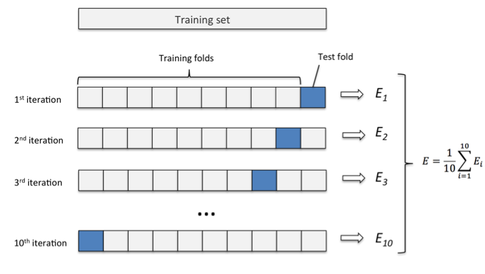
\includegraphics[width=4in]{k-fold.png}
\caption{K-fold cross validation schematic}
\end{figure}

\subsection{Necessary functions}\label{necessary-functions}

Before beginning, there are a few new functions to be familiar with.

\subsubsection{\texorpdfstring{\texttt{nest()} and
\texttt{unnest()}}{nest() and unnest()}}\label{nest-and-unnest}

The \texttt{tiydr::nest()} function converts rows of a dataframe into a
list, and stores this list in a column called \texttt{data}:

\begin{Shaded}
\begin{Highlighting}[]
\NormalTok{## To ensure "pretty printing", we must force our input dataframe to be a tibble:}
\NormalTok{iris2 <-}\StringTok{ }\KeywordTok{as.tibble}\NormalTok{(iris)}

\NormalTok{iris2 }\OperatorTok\StringTok{ }\KeywordTok{nest}\NormalTok{()}
\end{Highlighting}
\end{Shaded}

\begin{verbatim}
## # A tibble: 1 x 1
##                 data
##               <list>
## 1 <tibble [150 x 5]>
\end{verbatim}

You can further specify that certain columns \emph{not} be nested.

\begin{Shaded}
\begin{Highlighting}[]
\NormalTok{### Subtract Sepal.Width from nest() to preserve it}
\NormalTok{iris2 }\OperatorTok\StringTok{ }\KeywordTok{nest}\NormalTok{(}\OperatorTok{-}\NormalTok{Sepal.Width)}
\end{Highlighting}
\end{Shaded}

\begin{verbatim}
## # A tibble: 23 x 2
##    Sepal.Width              data
##          <dbl>            <list>
##  1         3.5  <tibble [6 x 4]>
##  2         3.0 <tibble [26 x 4]>
##  3         3.2 <tibble [13 x 4]>
##  4         3.1 <tibble [11 x 4]>
##  5         3.6  <tibble [4 x 4]>
##  6         3.9  <tibble [2 x 4]>
##  7         3.4 <tibble [12 x 4]>
##  8         2.9 <tibble [10 x 4]>
##  9         3.7  <tibble [3 x 4]>
## 10         4.0  <tibble [1 x 4]>
## # ... with 13 more rows
\end{verbatim}

In the above output, you can see that all rows corresponding to each
\texttt{Sepal.Length} value have been packaged into a list in a new
column called \texttt{data}, for later use.

The \texttt{tiydr::unnest()} undoes nestingL

\begin{Shaded}
\begin{Highlighting}[]
\NormalTok{iris2 }\OperatorTok\StringTok{ }
\StringTok{    }\KeywordTok{nest}\NormalTok{() }\OperatorTok\StringTok{  }\NormalTok{### make it all one column}
\StringTok{    }\KeywordTok{unnest}\NormalTok{() }\OperatorTok\StringTok{   }\NormalTok{### unnest to restore to original data frame state}
\StringTok{    }\KeywordTok{head}\NormalTok{()}
\end{Highlighting}
\end{Shaded}

\begin{verbatim}
## # A tibble: 6 x 5
##   Sepal.Length Sepal.Width Petal.Length Petal.Width Species
##          <dbl>       <dbl>        <dbl>       <dbl>  <fctr>
## 1          5.1         3.5          1.4         0.2  setosa
## 2          4.9         3.0          1.4         0.2  setosa
## 3          4.7         3.2          1.3         0.2  setosa
## 4          4.6         3.1          1.5         0.2  setosa
## 5          5.0         3.6          1.4         0.2  setosa
## 6          5.4         3.9          1.7         0.4  setosa
\end{verbatim}

\subsubsection{\texorpdfstring{\texttt{modelr::crossv\_kfold()}}{modelr::crossv\_kfold()}}\label{modelrcrossv_kfold}

This function uses random sampling to create K folds for you from a
given dataset and produces a data frame with three columns:

\begin{itemize}
\tightlist
\item
  \texttt{train}, the training fold
\item
  \texttt{test}, the associated testing fold
\item
  \texttt{.id}, the fold index for each train-test set. This column
  ranges from 1-K.
\end{itemize}

\begin{Shaded}
\begin{Highlighting}[]
\KeywordTok{set.seed}\NormalTok{(}\DecValTok{10392}\NormalTok{)}
\NormalTok{iris }\OperatorTok\StringTok{ }\KeywordTok{crossv_kfold}\NormalTok{(}\DecValTok{5}\NormalTok{)}
\end{Highlighting}
\end{Shaded}

\begin{verbatim}
## # A tibble: 5 x 3
##            train           test   .id
##           <list>         <list> <chr>
## 1 <S3: resample> <S3: resample>     1
## 2 <S3: resample> <S3: resample>     2
## 3 <S3: resample> <S3: resample>     3
## 4 <S3: resample> <S3: resample>     4
## 5 <S3: resample> <S3: resample>     5
\end{verbatim}

\subsubsection{\texorpdfstring{\texttt{broom::augment()}}{broom::augment()}}\label{broomaugment}

We have seen this function before along with \texttt{tidy()} and
\texttt{glance()}, but not really used it in depth. Now its utility is
revealed: This function merges, into a single dataframe, the input data
with the \textbf{fitted values} for a model, aka predictions! These
values are stored in a column called \texttt{.fitted}. Below, I show you
how you can directly see the true values of sepal length as well as what
the model predicts the sepal lengths would be, for the relevant petal
length.

\begin{Shaded}
\begin{Highlighting}[]
\NormalTok{fit <-}\StringTok{ }\KeywordTok{lm}\NormalTok{(Sepal.Length }\OperatorTok{~}\StringTok{ }\NormalTok{Petal.Length, }\DataTypeTok{data=}\NormalTok{iris)}
\KeywordTok{augment}\NormalTok{(fit) }\OperatorTok\StringTok{ }\KeywordTok{select}\NormalTok{(Sepal.Length, Petal.Length, .fitted) }\OperatorTok\StringTok{ }\KeywordTok{head}\NormalTok{()}
\end{Highlighting}
\end{Shaded}

\begin{verbatim}
##   Sepal.Length Petal.Length  .fitted
## 1          5.1          1.4 4.879095
## 2          4.9          1.4 4.879095
## 3          4.7          1.3 4.838202
## 4          4.6          1.5 4.919987
## 5          5.0          1.4 4.879095
## 6          5.4          1.7 5.001771
\end{verbatim}

\subsection{Performing cross validation on a linear
model}\label{performing-cross-validation-on-a-linear-model}

This section demonstrates how to run a k-fold cross validation for a
linear model. Specifically, we will validate the model:
\texttt{lm(Sepal.Length\ \textasciitilde{}\ Petal.Length\ +\ Species)}
with K=10 folds.

To begin, we will set the random seed to a random number of our
choosing:

\begin{Shaded}
\begin{Highlighting}[]
\KeywordTok{set.seed}\NormalTok{(}\DecValTok{1011}\NormalTok{)}
\end{Highlighting}
\end{Shaded}

Next, we create the K=10 folds and create 10 models on the
\texttt{train} column. Note that we have seen similar use of
\texttt{purrr:map()} when running permutation tests.

\begin{Shaded}
\begin{Highlighting}[]
\NormalTok{iris }\OperatorTok
\StringTok{  }\KeywordTok{crossv_kfold}\NormalTok{(}\DecValTok{10}\NormalTok{) }\OperatorTok
\StringTok{  }\KeywordTok{mutate}\NormalTok{(}\DataTypeTok{model =}\NormalTok{ purrr}\OperatorTok{::}\KeywordTok{map}\NormalTok{(train, }\OperatorTok{~}\KeywordTok{lm}\NormalTok{(Sepal.Length }\OperatorTok{~}\StringTok{ }\NormalTok{Petal.Length, }\DataTypeTok{data=}\NormalTok{.))) ->}\StringTok{ }\NormalTok{trained.models}

\NormalTok{trained.models}
\end{Highlighting}
\end{Shaded}

\begin{verbatim}
## # A tibble: 10 x 4
##             train           test   .id    model
##            <list>         <list> <chr>   <list>
##  1 <S3: resample> <S3: resample>    01 <S3: lm>
##  2 <S3: resample> <S3: resample>    02 <S3: lm>
##  3 <S3: resample> <S3: resample>    03 <S3: lm>
##  4 <S3: resample> <S3: resample>    04 <S3: lm>
##  5 <S3: resample> <S3: resample>    05 <S3: lm>
##  6 <S3: resample> <S3: resample>    06 <S3: lm>
##  7 <S3: resample> <S3: resample>    07 <S3: lm>
##  8 <S3: resample> <S3: resample>    08 <S3: lm>
##  9 <S3: resample> <S3: resample>    09 <S3: lm>
## 10 <S3: resample> <S3: resample>    10 <S3: lm>
\end{verbatim}

In the output, we see four columns:

\begin{itemize}
\tightlist
\item
  \texttt{train}, the training fold, produced by
  \texttt{crossv\_kfold()}
\item
  \texttt{test}, the associated testing fold, produced by
  \texttt{crossv\_kfold()}
\item
  \texttt{.id}, the fold index for each train-test set, produced by
  \texttt{crossv\_kfold()}
\item
  \texttt{model}, the fitted linear model, produced in the call to
  \texttt{purrr:map()}
\end{itemize}

Now, we need to evaluate each trained model on its respective test data.
Happily, \texttt{modelr} makes this easy with convenience functions
\texttt{rmse()}. This function takes two arguments as follows:
\texttt{rmse(fitted\ model,\ dataset)}. Therefore, in one call to
\texttt{rmse()}, we can calculate the RMSE from the trained model on the
test data.

To accomplish this, we need to use the function \texttt{purrr::map2()},
which is like \texttt{map()} but when there are two inputs to the
function of interest. We use this function as
\texttt{purrr::map2\_dbl()} to specify that we want numeric (double)
output:

\begin{Shaded}
\begin{Highlighting}[]
\KeywordTok{map2_dbl}\NormalTok{(trained.models}\OperatorTok{$}\NormalTok{model, trained.models}\OperatorTok{$}\NormalTok{test, rmse) ->}\StringTok{ }\NormalTok{test.rmse}

\NormalTok{test.rmse}
\end{Highlighting}
\end{Shaded}

\begin{verbatim}
##         1         2         3         4         5         6         7 
## 0.4294813 0.4220141 0.3264871 0.4495766 0.3919250 0.2986833 0.4156295 
##         8         9        10 
## 0.5210324 0.4468359 0.3500398
\end{verbatim}

These values correspond to the root mean square error of our model,
which can be interpretted as the error in model inferences. Recall, we
are predicting Sepal.Length in our model, which is distributed as:

\begin{Shaded}
\begin{Highlighting}[]
\KeywordTok{summary}\NormalTok{(iris}\OperatorTok{$}\NormalTok{Sepal.Length)}
\end{Highlighting}
\end{Shaded}

\begin{verbatim}
##    Min. 1st Qu.  Median    Mean 3rd Qu.    Max. 
##   4.300   5.100   5.800   5.843   6.400   7.900
\end{verbatim}

Compared to the range of values for Sepal.Lengths, our errors are rather
low (in the \textasciitilde{}10\% range), so our model is pretty good.
We can further run some summary statistics on the RMSE:

\begin{Shaded}
\begin{Highlighting}[]
\KeywordTok{summary}\NormalTok{(test.rmse)}
\end{Highlighting}
\end{Shaded}

\begin{verbatim}
##    Min. 1st Qu.  Median    Mean 3rd Qu.    Max. 
##  0.2987  0.3605  0.4188  0.4052  0.4425  0.5210
\end{verbatim}

\begin{Shaded}
\begin{Highlighting}[]
\KeywordTok{sd}\NormalTok{(test.rmse)}
\end{Highlighting}
\end{Shaded}

\begin{verbatim}
## [1] 0.06571102
\end{verbatim}

\begin{Shaded}
\begin{Highlighting}[]
\NormalTok{## Convert to data frame and plot:}
\KeywordTok{as.data.frame}\NormalTok{(test.rmse) }\OperatorTok\StringTok{ }\KeywordTok{ggplot}\NormalTok{(}\KeywordTok{aes}\NormalTok{(}\DataTypeTok{x=}\StringTok{""}\NormalTok{, }\DataTypeTok{y=}\NormalTok{test.rmse)) }\OperatorTok{+}\StringTok{ }\KeywordTok{geom_boxplot}\NormalTok{()}
\end{Highlighting}
\end{Shaded}

\begin{center}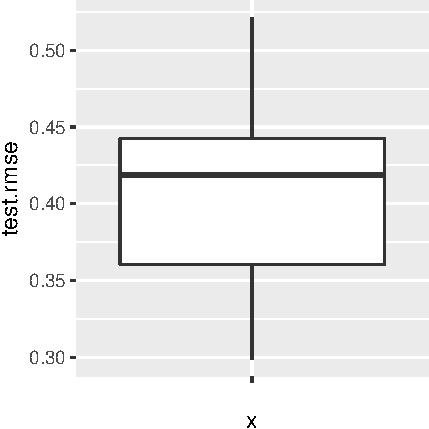
\includegraphics{kfold_supplement_files/figure-latex/unnamed-chunk-10-1} \end{center}

In the boxplot, there is one curious point (literally): the outlier
\textgreater{} 0.5. This point probably corresponds to a slightly
``pathological'' test set, i.e.~with different features from the rest of
the data.

Finally, we can compare our RMSE from the test data to RMSE from the
training data. If our model is robust, then these will have similar
distributions:

\begin{Shaded}
\begin{Highlighting}[]
\KeywordTok{map2_dbl}\NormalTok{(trained.models}\OperatorTok{$}\NormalTok{model, trained.models}\OperatorTok{$}\NormalTok{train, rmse) ->}\StringTok{ }\NormalTok{train.rmse}


\NormalTok{## Convert these to **vectors** to run the test below}
\KeywordTok{as.numeric}\NormalTok{(test.rmse) ->}\StringTok{ }\NormalTok{test.rmse2}
\KeywordTok{as.numeric}\NormalTok{(train.rmse) ->}\StringTok{ }\NormalTok{train.rmse2}


\NormalTok{## Run a test on train/test rmse, remembering that these are PAIRED by k-fold! }
\KeywordTok{wilcox.test}\NormalTok{(test.rmse2, train.rmse2, }\DataTypeTok{paired=}\NormalTok{T)}
\end{Highlighting}
\end{Shaded}

\begin{verbatim}
## 
##  Wilcoxon signed rank test
## 
## data:  test.rmse2 and train.rmse2
## V = 29, p-value = 0.9219
## alternative hypothesis: true location shift is not equal to 0
\end{verbatim}

A quick hypothesis test to compare distributions (Wilcoxon signed-rank)
gives P\textgreater{}0.05, suggesting that these RMSE values are from
the same underlying distribution and do not significantly differ. In
total, therefore, the K-fold cross validation showed us that we have a
fairly robust model.

\subsection{Performing cross validation on a logistic regression
model}\label{performing-cross-validation-on-a-logistic-regression-model}

The procedure for cross-validation is the same for any type of model,
but \texttt{modelr} does not have any convenience functions to summarize
validations (as in, \texttt{rmse()} above). Therefore, in this and other
such circumstances, we'll need to go through the full procedure of
predicting from our test data and evaluating the predictions directly.
Here, we will fit the logistic regression:
\texttt{glm(outcome\ \textasciitilde{}\ .,\ data\ =\ biopsy,\ family=binomial)},
as in class.

We begin in much the same way:

\begin{Shaded}
\begin{Highlighting}[]
\NormalTok{biopsy <-}\StringTok{ }\KeywordTok{read.csv}\NormalTok{(}\StringTok{"biopsy.csv"}\NormalTok{)}

\NormalTok{## Make the folds and train the models}
\NormalTok{biopsy }\OperatorTok
\StringTok{  }\KeywordTok{crossv_kfold}\NormalTok{(}\DecValTok{10}\NormalTok{) }\OperatorTok
\StringTok{  }\KeywordTok{mutate}\NormalTok{(}\DataTypeTok{model =}\NormalTok{ purrr}\OperatorTok{::}\KeywordTok{map}\NormalTok{(train, }\OperatorTok{~}\KeywordTok{glm}\NormalTok{(outcome }\OperatorTok{~}\StringTok{ }\NormalTok{., }\DataTypeTok{data=}\NormalTok{., }\DataTypeTok{family=}\NormalTok{binomial))) ->}\StringTok{ }\NormalTok{trained.models}

\NormalTok{trained.models}
\end{Highlighting}
\end{Shaded}

\begin{verbatim}
## # A tibble: 10 x 4
##             train           test   .id     model
##            <list>         <list> <chr>    <list>
##  1 <S3: resample> <S3: resample>    01 <S3: glm>
##  2 <S3: resample> <S3: resample>    02 <S3: glm>
##  3 <S3: resample> <S3: resample>    03 <S3: glm>
##  4 <S3: resample> <S3: resample>    04 <S3: glm>
##  5 <S3: resample> <S3: resample>    05 <S3: glm>
##  6 <S3: resample> <S3: resample>    06 <S3: glm>
##  7 <S3: resample> <S3: resample>    07 <S3: glm>
##  8 <S3: resample> <S3: resample>    08 <S3: glm>
##  9 <S3: resample> <S3: resample>    09 <S3: glm>
## 10 <S3: resample> <S3: resample>    10 <S3: glm>
\end{verbatim}

Again, we have our training and test data, their associated IDs, and the
models fit to the training data. We now must actually grab predictions
out of test, using some \texttt{tidyverse} magic with the
\texttt{unnest()} and \texttt{map2()} functions. We want to run
\texttt{predict()}, as usual, with the testing data in the \texttt{test}
column with the trained models in \texttt{model} column. We use
\texttt{map2()} to send both these inputs into \texttt{predict()} (with
\texttt{type\ =\ "response"} to actually get predicted probabilities),
and we shove the whole thing into \texttt{unnest()} to reveal the
output.

\begin{Shaded}
\begin{Highlighting}[]
\NormalTok{trained.models }\OperatorTok\StringTok{ }
\StringTok{  }\KeywordTok{unnest}\NormalTok{( }\DataTypeTok{pred =} \KeywordTok{map2}\NormalTok{( model, test, }\OperatorTok{~}\KeywordTok{predict}\NormalTok{( .x, .y, }\DataTypeTok{type =} \StringTok{"response"}\NormalTok{)) ) ->}\StringTok{ }\NormalTok{test.predictions}

\NormalTok{test.predictions}
\end{Highlighting}
\end{Shaded}

\begin{verbatim}
## # A tibble: 683 x 2
##      .id        pred
##    <chr>       <dbl>
##  1    01 0.014053295
##  2    01 0.655229137
##  3    01 0.008765455
##  4    01 0.009482819
##  5    01 0.684536415
##  6    01 0.998284067
##  7    01 0.999754059
##  8    01 0.976952451
##  9    01 0.568713564
## 10    01 0.999989396
## # ... with 673 more rows
\end{verbatim}

Our output here is a data frame where, for each row in each dataset (see
the \texttt{.id} column!), we have predicted the probability of
malignancy. In order to evaluate the model, we must compare these
results to the \textbf{true} outcome in the test data. To do this, we
need to modify our last line of code a little bit. We will include the
function \texttt{broom::augment()} to get everything in one go. Recall:
\texttt{augment()} not only does predictions, it also shows them in
relation to the actual data (true outcome!). Therefore, we mainly use
\texttt{augment()} to grab the \texttt{outcome} column from the test
data. The function will do predictions as well (like the
\texttt{predict()} line), but it will give us the
\emph{linear.predictors} when we really want the \emph{fitted.values},
so we keep \texttt{predict()}.

\begin{Shaded}
\begin{Highlighting}[]
\NormalTok{trained.models }\OperatorTok\StringTok{ }
\StringTok{  }\KeywordTok{unnest}\NormalTok{( }\DataTypeTok{fitted =} \KeywordTok{map2}\NormalTok{(model, test, }\OperatorTok{~}\KeywordTok{augment}\NormalTok{(.x, }\DataTypeTok{newdata =}\NormalTok{ .y)),          }
  \DataTypeTok{pred =} \KeywordTok{map2}\NormalTok{( model, test, }\OperatorTok{~}\KeywordTok{predict}\NormalTok{( .x, .y, }\DataTypeTok{type =} \StringTok{"response"}\NormalTok{)) ) ->}\StringTok{ }\NormalTok{test.predictions}

\NormalTok{test.predictions }\OperatorTok\StringTok{ }\KeywordTok{select}\NormalTok{(.id, outcome, pred )}
\end{Highlighting}
\end{Shaded}

\begin{verbatim}
## # A tibble: 683 x 3
##      .id   outcome        pred
##    <chr>    <fctr>       <dbl>
##  1    01    benign 0.014053295
##  2    01 malignant 0.655229137
##  3    01    benign 0.008765455
##  4    01    benign 0.009482819
##  5    01 malignant 0.684536415
##  6    01 malignant 0.998284067
##  7    01 malignant 0.999754059
##  8    01 malignant 0.976952451
##  9    01 malignant 0.568713564
## 10    01 malignant 0.999989396
## # ... with 673 more rows
\end{verbatim}

Behold: A data frame with three columns:

\begin{itemize}
\tightlist
\item
  \texttt{.id}, the fold 1-10
\item
  \texttt{outcome}, the TRUE outcome known from the test data
\item
  \texttt{pred}, the PREDICTED probability of malignancy for the test
  data using the respective Kth training model
\end{itemize}

We can use this outcome to get an AUC for all testing folds, using the
\texttt{pROC::roc()} function on columns in the dataframe:

\begin{Shaded}
\begin{Highlighting}[]
\NormalTok{test.predictions }\OperatorTok\StringTok{ }
\StringTok{    }\KeywordTok{group_by}\NormalTok{(.id) }\OperatorTok
\StringTok{    }\KeywordTok{summarize}\NormalTok{(}\DataTypeTok{auc =} \KeywordTok{roc}\NormalTok{(outcome, .fitted)}\OperatorTok{$}\NormalTok{auc) }\OperatorTok\StringTok{  }
\StringTok{    }\KeywordTok{select}\NormalTok{(auc)}
\end{Highlighting}
\end{Shaded}

\begin{verbatim}
## # A tibble: 10 x 1
##          auc
##        <dbl>
##  1 0.9990909
##  2 0.9888889
##  3 0.9968421
##  4 0.9922705
##  5 0.9857955
##  6 1.0000000
##  7 0.9935897
##  8 1.0000000
##  9 0.9973214
## 10 0.9949341
\end{verbatim}

Now, these are some insanely high AUC's (all \textgreater{}= 0.98!),
showing that we have a great model here. Does the training data show
something similar? Let's find out using the same procedure we used to
fit the test data - we simply replace the \texttt{test} column with the
\texttt{train} column:

\begin{Shaded}
\begin{Highlighting}[]
\NormalTok{train.predictions <-}\StringTok{ }\NormalTok{trained.models }\OperatorTok\StringTok{ }\KeywordTok{unnest}\NormalTok{(  }\DataTypeTok{fitted =} \KeywordTok{map2}\NormalTok{(model, train, }\OperatorTok{~}\KeywordTok{augment}\NormalTok{(.x, }\DataTypeTok{newdata =}\NormalTok{ .y)),          }
                                                \DataTypeTok{pred =} \KeywordTok{map2}\NormalTok{( model, train, }\OperatorTok{~}\KeywordTok{predict}\NormalTok{( .x, .y, }\DataTypeTok{type =} \StringTok{"response"}\NormalTok{)) )}

\NormalTok{train.predictions }\OperatorTok\StringTok{ }
\StringTok{  }\KeywordTok{group_by}\NormalTok{(.id) }\OperatorTok
\StringTok{  }\KeywordTok{summarize}\NormalTok{(}\DataTypeTok{auc =} \KeywordTok{roc}\NormalTok{(outcome, .fitted)}\OperatorTok{$}\NormalTok{auc) }\OperatorTok\StringTok{  }\NormalTok{### outcome from the true data, .fitted from augment's output. Run roc() on these columns and pull out $auc!}
\StringTok{  }\KeywordTok{select}\NormalTok{(auc)}
\end{Highlighting}
\end{Shaded}

\begin{verbatim}
## # A tibble: 10 x 1
##          auc
##        <dbl>
##  1 0.9961098
##  2 0.9971557
##  3 0.9962044
##  4 0.9967511
##  5 0.9967209
##  6 0.9959387
##  7 0.9964030
##  8 0.9959196
##  9 0.9961288
## 10 0.9961754
\end{verbatim}

Just as good! We are confirmed that the training and testing data give
similar predictions (a nearly perfect model).

\paragraph{More advanced}\label{more-advanced}

Not satified with just AUC and wanting some confusion matrix measures
across folds? Here some complex but fantastic \texttt{tidyverse} magic
to get you there.

First, we need to convert the predicted test probabilities to
predictions, assuming a cutoff of 0.5. We also need to summarize
predictions across folds:

\begin{Shaded}
\begin{Highlighting}[]
\NormalTok{## How to change pred column from probability to real prediction}
\NormalTok{test.predictions }\OperatorTok\StringTok{ }
\StringTok{  }\KeywordTok{select}\NormalTok{(.id, outcome, pred ) }\OperatorTok
\StringTok{  }\KeywordTok{mutate}\NormalTok{(}\DataTypeTok{pred =} \KeywordTok{ifelse}\NormalTok{(pred }\OperatorTok{>=}\StringTok{ }\FloatTok{0.5}\NormalTok{, }\StringTok{"malignant"}\NormalTok{, }\StringTok{"benign"}\NormalTok{))}
\end{Highlighting}
\end{Shaded}

\begin{verbatim}
## # A tibble: 683 x 3
##      .id   outcome      pred
##    <chr>    <fctr>     <chr>
##  1    01    benign    benign
##  2    01 malignant malignant
##  3    01    benign    benign
##  4    01    benign    benign
##  5    01 malignant malignant
##  6    01 malignant malignant
##  7    01 malignant malignant
##  8    01 malignant malignant
##  9    01 malignant malignant
## 10    01 malignant malignant
## # ... with 673 more rows
\end{verbatim}

\begin{Shaded}
\begin{Highlighting}[]
\NormalTok{## Tally it all up by fold}
\NormalTok{test.predictions }\OperatorTok\StringTok{ }
\StringTok{  }\KeywordTok{select}\NormalTok{(.id, outcome, pred ) }\OperatorTok
\StringTok{  }\KeywordTok{mutate}\NormalTok{(}\DataTypeTok{pred =} \KeywordTok{ifelse}\NormalTok{(pred }\OperatorTok{>=}\StringTok{ }\FloatTok{0.5}\NormalTok{, }\StringTok{"malignant"}\NormalTok{, }\StringTok{"benign"}\NormalTok{)) }\OperatorTok
\StringTok{  }\KeywordTok{group_by}\NormalTok{(.id, outcome, pred) }\OperatorTok\StringTok{ }\KeywordTok{tally}\NormalTok{()}
\end{Highlighting}
\end{Shaded}

\begin{verbatim}
## # A tibble: 33 x 4
## # Groups:   .id, outcome [?]
##      .id   outcome      pred     n
##    <chr>    <fctr>     <chr> <int>
##  1    01    benign    benign    44
##  2    01 malignant    benign     1
##  3    01 malignant malignant    24
##  4    02    benign    benign    44
##  5    02    benign malignant     1
##  6    02 malignant    benign     2
##  7    02 malignant malignant    22
##  8    03    benign    benign    48
##  9    03    benign malignant     2
## 10    03 malignant    benign     1
## # ... with 23 more rows
\end{verbatim}

Here's what we see, for fold 1:

\begin{itemize}
\tightlist
\item
  There are 38 benign predictions for benign patients, making \textbf{38
  true negatives}
\item
  There are 2 benign predictions for malignant patients, making
  \textbf{2 false negatives}
\item
  There are 29 malignant predictions for malignant patients, making
  \textbf{29 true positive}
\item
  There are 0 malignant predictions for benign patients, making
  \textbf{0 false positives}
\end{itemize}

Therefore, for fold 1, the True Positive rate is 29/(29+2) = 0.935.

We can do this for all K's with a lot of (complicated but awesome)
magic. I \textbf{strongly recommed} playing around with this code, line
by line, until you understand what it does. Note in particular the
\texttt{mutate()} line, which cycles through various conditions in order
to assign either as True Positive (TP), FP, TN, or FN.

\begin{Shaded}
\begin{Highlighting}[]
\NormalTok{## Create a dataframe confusion matrix}
\NormalTok{test.predictions }\OperatorTok\StringTok{ }
\StringTok{  }\KeywordTok{select}\NormalTok{(.id, outcome, pred ) }\OperatorTok
\StringTok{  }\KeywordTok{mutate}\NormalTok{(}\DataTypeTok{pred =} \KeywordTok{ifelse}\NormalTok{(pred }\OperatorTok{>=}\StringTok{ }\FloatTok{0.5}\NormalTok{, }\StringTok{"malignant"}\NormalTok{, }\StringTok{"benign"}\NormalTok{)) }\OperatorTok
\StringTok{  }\KeywordTok{group_by}\NormalTok{(.id, outcome, pred) }\OperatorTok\StringTok{ }
\StringTok{  }\KeywordTok{tally}\NormalTok{() }\OperatorTok
\StringTok{  }\KeywordTok{mutate}\NormalTok{(}\DataTypeTok{class =}  \KeywordTok{ifelse}\NormalTok{(outcome }\OperatorTok{==}\StringTok{ }\NormalTok{pred }\OperatorTok{&}\StringTok{ }\NormalTok{pred }\OperatorTok{==}\StringTok{ "malignant"}\NormalTok{, }\StringTok{"TP"}\NormalTok{,            }
                  \KeywordTok{ifelse}\NormalTok{(outcome }\OperatorTok{!=}\StringTok{ }\NormalTok{pred }\OperatorTok{&}\StringTok{ }\NormalTok{pred }\OperatorTok{==}\StringTok{ "malignant"}\NormalTok{, }\StringTok{"FP"}\NormalTok{,            }
                  \KeywordTok{ifelse}\NormalTok{(outcome }\OperatorTok{==}\StringTok{ }\NormalTok{pred }\OperatorTok{&}\StringTok{ }\NormalTok{pred }\OperatorTok{==}\StringTok{ "benign"}\NormalTok{, }\StringTok{"TN"}\NormalTok{, }\StringTok{"FN"}\NormalTok{)))) }\OperatorTok
\StringTok{  }\KeywordTok{ungroup}\NormalTok{() }\OperatorTok\StringTok{  }\NormalTok{### We want to ditch the `outcome` column, so remove it from grouping}
\StringTok{  }\KeywordTok{select}\NormalTok{(.id, n, class) }\OperatorTok\StringTok{  }\NormalTok{### Retain only columns of interest; use spread to get a column per classification type}
\StringTok{  }\KeywordTok{spread}\NormalTok{(class, n) ->}\StringTok{ }\NormalTok{confusion}

\NormalTok{confusion}
\end{Highlighting}
\end{Shaded}

\begin{verbatim}
## # A tibble: 10 x 5
##      .id    FN    FP    TN    TP
##  * <chr> <int> <int> <int> <int>
##  1    01     1    NA    44    24
##  2    02     2     1    44    22
##  3    03     1     2    48    18
##  4    04     2     2    43    21
##  5    05     4     3    41    20
##  6    06    NA    NA    36    32
##  7    07    NA     1    41    26
##  8    08     1    NA    51    16
##  9    09    NA     1    39    28
## 10    10     2    NA    47    19
\end{verbatim}

\begin{Shaded}
\begin{Highlighting}[]
\NormalTok{## Use the tidyr::replace_na() function to replace all NA's in columns TP, TN, FP, FN with 0:}
\NormalTok{confusion <-}\StringTok{ }\KeywordTok{replace_na}\NormalTok{(confusion, }\KeywordTok{list}\NormalTok{(}\DataTypeTok{TP=}\DecValTok{0}\NormalTok{, }\DataTypeTok{TN=}\DecValTok{0}\NormalTok{, }\DataTypeTok{FP=}\DecValTok{0}\NormalTok{, }\DataTypeTok{FN=}\DecValTok{0}\NormalTok{))}
\NormalTok{confusion}
\end{Highlighting}
\end{Shaded}

\begin{verbatim}
## # A tibble: 10 x 5
##      .id    FN    FP    TN    TP
##  * <chr> <dbl> <dbl> <dbl> <dbl>
##  1    01     1     0    44    24
##  2    02     2     1    44    22
##  3    03     1     2    48    18
##  4    04     2     2    43    21
##  5    05     4     3    41    20
##  6    06     0     0    36    32
##  7    07     0     1    41    26
##  8    08     1     0    51    16
##  9    09     0     1    39    28
## 10    10     2     0    47    19
\end{verbatim}

\begin{Shaded}
\begin{Highlighting}[]
\NormalTok{## Some classifer metric across all folds}
\NormalTok{confusion }\OperatorTok
\StringTok{  }\KeywordTok{group_by}\NormalTok{(.id) }\OperatorTok
\StringTok{  }\KeywordTok{summarize}\NormalTok{(}\DataTypeTok{TPR     =}\NormalTok{ TP}\OperatorTok{/}\NormalTok{(TP}\OperatorTok{+}\NormalTok{FN),}
            \DataTypeTok{Accuracy =}\NormalTok{ (TP}\OperatorTok{+}\NormalTok{TN)}\OperatorTok{/}\NormalTok{(TP}\OperatorTok{+}\NormalTok{TN}\OperatorTok{+}\NormalTok{FP}\OperatorTok{+}\NormalTok{FN),}
            \DataTypeTok{PPV      =}\NormalTok{ TP}\OperatorTok{/}\NormalTok{(TP}\OperatorTok{+}\NormalTok{FP)) ->}\StringTok{ }\NormalTok{fold.metrics}

\NormalTok{fold.metrics}
\end{Highlighting}
\end{Shaded}

\begin{verbatim}
## # A tibble: 10 x 4
##      .id       TPR  Accuracy       PPV
##    <chr>     <dbl>     <dbl>     <dbl>
##  1    01 0.9600000 0.9855072 1.0000000
##  2    02 0.9166667 0.9565217 0.9565217
##  3    03 0.9473684 0.9565217 0.9000000
##  4    04 0.9130435 0.9411765 0.9130435
##  5    05 0.8333333 0.8970588 0.8695652
##  6    06 1.0000000 1.0000000 1.0000000
##  7    07 1.0000000 0.9852941 0.9629630
##  8    08 0.9411765 0.9852941 1.0000000
##  9    09 1.0000000 0.9852941 0.9655172
## 10    10 0.9047619 0.9705882 1.0000000
\end{verbatim}

\begin{Shaded}
\begin{Highlighting}[]
\NormalTok{## Finally we can summarize:}
\NormalTok{fold.metrics }\OperatorTok\StringTok{ }\KeywordTok{summarize}\NormalTok{(}\DataTypeTok{meanTPR =} \KeywordTok{mean}\NormalTok{(TPR), }\DataTypeTok{meanAcc =} \KeywordTok{mean}\NormalTok{(Accuracy), }\DataTypeTok{meanPPV=}\KeywordTok{mean}\NormalTok{(PPV))}
\end{Highlighting}
\end{Shaded}

\begin{verbatim}
## # A tibble: 1 x 3
##    meanTPR   meanAcc   meanPPV
##      <dbl>     <dbl>     <dbl>
## 1 0.941635 0.9663257 0.9567611
\end{verbatim}

\textbf{At long last}, our K-fold validation gave us a mean TPR of 0.95,
mean accuracy of 0.966, and mean positive predictive of 0.95. Together,
this all points to a very good model.


\end{document}
